\documentclass{amsart}

\usepackage[top = 1in, bottom = 1in, left =1in, right = 1in]{geometry}

\usepackage{packages} % Look here for packages before you add more, place all figures in Figures folder
\usepackage{macros} % Check here for macros before you add more

\usepackage{hyperref}
\usepackage{pdfpages}


\newcommand{\prob}{\mathbb{P}} % Probabliity symbol
\newcommand{\iid}{\overset{\mathrm{iid}}{\sim}} % IID symbol

\usepackage{setspace}
	\doublespacing

\begin{comment}
	!!!!!!!!!!!!!!!!!!!!!!!!!!!!!!!!!!!!!!!!!!!!
	Add each section to a different tex file and use input to add content

	See intro for a template
	!!!!!!!!!!!!!!!!!!!!!!!!!!!!!!!!!!!!!!!!!!!!
\end{comment}

\title{Recurrent Switching Linear Dynamical Systems}
\author{Charbel Abi Younes \and Marvyn Bailly \and Bart Boom \and Rohin Gilman \and Daran Xu}
\date{}

\begin{document}

\begin{abstract}
	We investigate the modeling of complex dynamical systems using switching linear dynamical systems and recurrent switching linear dynamical systems. The literature shows that this method is able to estimate complex nonlinear dynamics, with an increase in performance by extending the SLDS to recurrent SLDS. The goal of this paper is to investigate if this model is able to capture the behavior of bifurcations effectively. To investigate this examine various systems where we know the dynamics. 
\end{abstract}

\maketitle

%%%%%%%%%%%%%%%%%%%%%%%%%%%%%%%%%%%%%%%%%%%%%%%%%%%%%%%
% Make sure to add any new macros to the final report 
% to ensure that they do not conflict with existsing
% ones.
%%%%%%%%%%%%%%%%%%%%%%%%%%%%%%%%%%%%%%%%%%%%%%%%%%%%%%%

\section{Introduction}

Consider a basketball player coming the court. They arrive at the three point line and have a decision to make: should they cut to the basket or run to the left corner. Depending on the positions of other players, the state in the game, or whether they are playing at home or away, the player might make a different decision. Scenarios like these produce data generated by complex, nonlinear dynamical systems. Instead of trying to produce the exact equations that lead to dynamics like those described above, we can instead understand these systems by decomposing them into multiple, simpler dynamical systems.

\begin{comment}
The literature shows that this method is able to estimate complex nonlinear dynamics. With an increase in performance by extending the SLDS to recursive SLDS (rSLDS). The goal of this paper is to investigate if rSLDS is able to capture bifurcations efficiently. To investigate this we take a look at different systems where we know the dynamics and the bifurcations in it. There is chosen to look at a hopf bifurcation in the Van der Pol oscillator additionally we studied the normal for of a Bautin bifurcation. 


The report is structured in the following manner, below we introduce the mathematical frame work and findings described in the paper. Section 2 we reproduce some results presented in the paper. The third section our results to the our investigation on bifurcation is presented and finally Section 4 concludes our findings and discusses limitations and potential future research directions.
\end{comment}

\subsection{Switching Linear Dynamical Systems}

Switching linear dynamical systems (SLDSs) are used to split up complex, nonlinear dynamical system data into a set of linear models. By fitting the data to an SLDS, a nonlinear representation is learned. Given sufficient data and an adequate number of linear models, it can learn the global dynamics of the system.

An SLDS has the following components for each time step $t = 1,2, \dots, T$: a discrete latent state $z_t$, a continuous latent state $x_t$, and an observation $y_t$. The underlying state $z_t$ is in the set $\brac{1,2,\dots,K}$ and is driven by a Markov process:
\[\prob(z_{t+1} = j \mid z_t = i) = \pi_{ij}, \]
where $\brak{\pi_{ij}}_{K\times K}$ is the transition matrix of the process. The underlying continuous state $x_t$ is in $\R^M$ and is driven by conditionally linear dynamics, dependent on the discrete latent state $z_{t+1}$:
\[x_{t+1} = A_{z_{t+1}} x_t + b_{z_{t+1}} + v_t, \]
where $A_k\in\R^{M\times M}$, $b_k\in \R^M$, and $v_t \iid \mathcal{N}(0,Q_{z_{t+1}})$, where $Q_k\in\R^{M\times M}$ is the covariance matrix of the normal distribution. Finally, the observation $y_t$ is generated from the corresponding discrete continuous and discrete latent states:
\[y_t = C_{z_{t}} x_t + d_{z_{t}} + w_t,\]
where $C_k\in\R^{N\times M}$, $d_k\in \R^N$, and $w_t \iid \mathcal{N}(0,S_{z_{t}})$, where $S_k\in\R^{N\times N}$ is the covariance matrix of the normal distribution.

The library of the linear systems involved in the SLDS is denoted by
\[\theta = \brac{\pi_k, A_k, b_k, Q_k, C_k, d_k, S_k \mid k = 1, \dots, K}.\]

\subsection{Fitting SLDSs}
%%%%%%%%%%%%%%%%%%%%%%%%%%%%%%%%%%%%%%%%%%
%%%%%%%%%%%%%%%%%%%%%%%%%%%%%%%%%%%%%%%%%%
%%%%%%%%%%%%%%%%%%%%%%%%%%%%%%%%%%%%%%%%%%
%%%%%%%%%%%%%%%%%%%%%%%%%%%%%%%%%%%%%%%%%%
%%%%%%%%%%%%%BELOW%%%%%%%%%%%%%%%%%%%%%%%%
%%%%%%%%%%%%%%%%%%%%%%%%%%%%%%%%%%%%%%%%%%
%%%%%%%%%%%%%%%%%%%%%%%%%%%%%%%%%%%%%%%%%%
%%%%%%%%%%%%%%%%%%%%%%%%%%%%%%%%%%%%%%%%%%
%%%%%%%%%%%%%%%%%%%%%%%%%%%%%%%%%%%%%%%%%%
%\textcolor{red}{Talk about message passing generating samples, and updating parameters after obtaining the samples}

%\subsubsection{Bayesian Inference using Gibbs Sampling}
  

The most common way to perform Bayesian inference is to use Gibbs sampling, which is an iterative method that updates our belief in the parameters $\theta$, continuous latent variables $\{x_{t}\}_{t=1:T}$, and the discrete latent variable $\{z_t\}_{t=1:T}$. At each iteration, we draw a sample from the conditional distribution of each variable based on the current samples of the other two variables. After convergence, we end up with estimations of $\theta$, $\{x_{t}\}_{t=1:T}$ and $\{z_t\}_{t=1:T}$:
\begin{enumerate}
  \item Sample $\theta$ from $\prob(\theta \mid \{z_t\}_{t=1:T}, \{x_{t}\}_{t=1:T})$
  \item Sample $\{x_t\}$ from $\prob(\{x_{t}\}_{t=1:T} \mid \{z_t\}_{t=1:T}, \theta)$
  \item Sample $\{z_t\}$ from $\prob(\{z_{t}\}_{t=1:T} \mid \{x_t\}_{t=1:T}, \theta)$
 \item Repeat steps (1-3) 
\end{enumerate}
The parameters sampling can be efficiently performed by the choosing appropriate prior distrbutions, to ensure the posterior has a closed-form expression, forming a conjugate pair between the prior and the posterior.
 
For simplicity, $C, S$, and $d$ are assumed to be same for all discrete states. To perform Bayesian inference efficiently, we assume conjugate Dirichlet priors for each row of the transition matrix $\pi_{k}$, and conjugate matrix normal inverse Wishart (MNIW) priors for the dynamical system parameters $\left(A_{k}, b_{k}\right), Q_{k}$:
$$
\begin{gathered}
\pi_{k}\left|\alpha \stackrel{\mathrm{iid}}{\sim} \operatorname{Dir}(\alpha), \quad\left(A_{k}, b_{k}\right), Q_{k}\right| \lambda \stackrel{\mathrm{iid}}{\sim} \operatorname{MNIW}(\lambda), \\
\left(C, d\right), S \mid \eta \stackrel{\mathrm{iid}}{\sim} \operatorname{MNIW}(\eta),
\end{gathered}
$$
where $\alpha, \lambda$, and $\eta$ denote hyperparameters. 
Given the samples latent states and observations, the posterior $\prob(\theta \mid \{z_t\}_{t=1:T}, \{x_{t}\}_{t=1:T})$ benefit from simple conjugate updates. 

%\subsubsection{Message Passing}    

Meanwhile, to obtain conditional samples of $\{x_t\}$ from $\prob(\{x_{t}\}_{t=1:T} \mid \{z_t\}_{t=1:T}, \theta)$, and $\{z_t\}$ from $\prob(\{z_{t}\}_{t=1:T} \mid \{x_t\}_{t=1:T}, \theta)$, one can use the message passing algorithm.

We start with considering the  conditional  density  of  the  latent continuous  state  sequence $x_{1:T}$ given  all  other  variables. Here we introduce the notation of potential: $\psi$ maps two states or three to a nonnegative value, such that $\psi(x_t,y_t)\propto \prob(y_t \mid x_t)$ and $\psi(x_t,x_{t+1},z_{t+1})\propto \prob(x_{t+1} \mid x_t,z_{t+1})$. This notation allows us to manipulate the conditional probability and the joint probability without worrying about the normalization terms. Following this notation and the graphical model of SLDS, the conditional density of $x_{1:T}$ can be expressed as $
\prod_{t=1}^{T-1} \psi\left(x_{t}, x_{t+1}, z_{t+1}\right) \psi\left(x_{t}, z_{t+1}\right) \prod_{t=1}^{T} \psi\left(x_{t}, y_{t}\right),
$

%The "message" defined as the sum of the messages from 
%\[m_{ji}(x_i) = \sum_{x_j} \psi_{ij}(x_i, x_j) \prod_{k \in \eta(j) \backslash \{i\}} m_{kj}(x_j)\]
 
%For the initial state $x_0$, we set $m_{0 \rightarrow 1}(x_1)=\psi(x_1,y_1)?????$. 
For $t\geq 2$,the message from time $t$ to time $t+1$, deonted $m_{t \rightarrow t+1}(x_{t+1})$, is computed as 
$ m_{t \rightarrow t+1}(x_{t+1})=\int \psi(x_t,y_t) \psi(x_t,x_{t+1},z_{t+1}) m_{t-1 \rightarrow t}(x_t) dx_t $. The paper does not clarify how to define the initial message $m_{0 \rightarrow 1}(x_1)$. I propose defining it as $m_{0 \rightarrow 1}(x_1)=\psi\left(x_{1}, z_{1}\right) \psi\left(x_{1}, y_{1}\right)$. Given that $x_{1:T}$ is  conditionally Gaussian given $z_{1:T}$ and $y_{1:T}$, these message passing integrasl will have closed forms, allowing us to perform forward propagation to evaluate $m_{0 \rightarrow 1}(x_1), m_{1 \rightarrow 2}(x_2),\dots, m_{T-1 \rightarrow T}(x_T)$. After that, one can perform the sampling of $\{x_t\}_{t=1:T}$ in a backward manner: 
\begin{itemize}
  \item Sample $x_T$ from $m_{T-1 \rightarrow T}(x_T)$, $z_{1:T}$ and $y_{1:T}$
  \item Sample $x_{T-1}$ from $m_{T-2 \rightarrow T-1}(x_{T-1})$ and the sampled $x_T$, $z_{1:T}$ and $y_{1:T}$
  \item Sample $x_{T-2}$ from $m_{T-3 \rightarrow T-2}(x_{T-2})$ and the sampled $x_{T-1}$, $z_{1:T}$ and $y_{1:T}$
  \item continue until getting the sample of $x_1$
\end{itemize}
After completing this forward-backward procedure, we obtain samples of $\{x_t\}$ conditioning on $\{z_t\}_{t=1:T}$, parameters $\theta$, and the observation $\{y_t\}_{t=1:T}$. Addtionally, we can generate samples for $z_t$ using a discrete version of this message passing algrithm. These complete one iteration of the Gibbs sampling process.


%%%%%%%%%%%%%%%%%%%%%%%%%%%%%%%%%%%%%%%%%%
%%%%%%%%%%%%%%%%%%%%%%%%%%%%%%%%%%%%%%%%%%
%%%%%%%%%%%%%%%%%%%%%%%%%%%%%%%%%%%%%%%%%%
%%%%%%%%%%%%%%%%%%%%%%%%%%%%%%%%%%%%%%%%%%
%%%%%%%%%%%%%%%%ABOVE%%%%%%%%%%%%%%%%%%%%%
%%%%%%%%%%%%%%%%%%%%%%%%%%%%%%%%%%%%%%%%%%
%%%%%%%%%%%%%%%%%%%%%%%%%%%%%%%%%%%%%%%%%%
%%%%%%%%%%%%%%%%%%%%%%%%%%%%%%%%%%%%%%%%%%

\subsection{Recurrent Switching Linear Dynamical Systems (rSLDSs)}

If a switch in the discrete state of a system should occur when the trajectory enters (or leaves) a particular region, the model will be unable to capture this behavior since the discrete state is a function only of the previous discrete state. To rectify this, we instead consider a recurrent switching linear dynamical system (rSLDS). 

The key difference between an SLDS and an rSLDS is in the update of the  discrete latent state, $z_t$. Instead of depending only on the previous discrete state, the update also depends on the continuous latent variable $x_t$. We can see this difference in dependencies Figure \ref{rSLDS}.

\begin{figure}[h!]
	\centering
	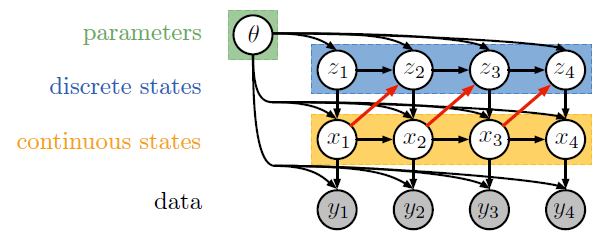
\includegraphics[width=0.5\textwidth]{rSLDS_diagram.png}
	\caption{The black arrows represent the dependencies of a tradidional SLDS, and the red arrows represent the added dependencies of an rSLDS.}
	\label{rSLDS}
\end{figure}

\textcolor{blue}{be aware, the stickbreaking is here!}

In the proposed model in the paper, the generation of discrete states $z_{t}$ follows:
$$
\begin{aligned}
z_{t+1} \mid z_{t}, x_{t},\left\{R_{k}, r_{k}\right\} & \sim \pi_{\mathrm{SB}}\left(\nu_{t+1}\right), \\
\nu_{t+1} & =R_{z_{t}} x_{t}+r_{z_{t}},
\end{aligned}
$$

where $R_{k} \in \mathbb{R}^{K-1 \times M}$ represents a weight matrix that specifies the recurrent dependencies, and $r_{k} \in \mathbb{R}^{K-1}$ is a bias that captures the Markov dependence of $z_{t+1}$ on $z_{t}$. The function $\pi_{\mathrm{SB}}: \mathbb{R}^{K-1} \rightarrow[0,1]^{K}$ maps a real vector to a normalized probability vector using the stick-breaking process, defined as follows:
$$
\begin{gathered}
\pi_{\mathrm{SB}}(\nu)=\left(\begin{array}{lll}
\pi_{\mathrm{SB}}^{(1)}(\nu) & \cdots & \pi_{\mathrm{SB}}^{(K)}(\nu)
\end{array}\right), \\
\pi_{\mathrm{SB}}^{(k)}(\nu)=\sigma\left(\nu_{k}\right) \prod_{j<k}\left(1-\sigma\left(\nu_{j}\right)\right)=\sigma\left(\nu_{k}\right) \prod_{j<k} \sigma\left(-\nu_{j}\right),
\end{gathered}
$$
for $k=1,2, \ldots, K-1$ and $\pi_{\mathrm{SB}}^{(K)}(\nu)=\prod_{k=1}^{K} \sigma\left(-\nu_{k}\right)$, where $\sigma(x)=e^{x} /\left(1+e^{x}\right)$ denotes the logistic function. The rest of the generative process of the rSLDS follows that of the SLDS. 

\subsection{Fitting rSLDSs} 
%%%%%%%%%%%%%%%%%%%%%%%%%%%%%%%%%%%%%%%%%%
%%%%%%%%%%%%%%%%%%%%%%%%%%%%%%%%%%%%%%%%%%
%%%%%%%%%%%%%%%%%%%%%%%%%%%%%%%%%%%%%%%%%%
%%%%%%%%%%%%%%%%%%%%%%%%%%%%%%%%%%%%%%%%%%
%%%%%%%%%%%%%BELOW%%%%%%%%%%%%%%%%%%%%%%%%
%%%%%%%%%%%%%%%%%%%%%%%%%%%%%%%%%%%%%%%%%%
%%%%%%%%%%%%%%%%%%%%%%%%%%%%%%%%%%%%%%%%%%
%%%%%%%%%%%%%%%%%%%%%%%%%%%%%%%%%%%%%%%%%%
%%%%%%%%%%%%%%%%%%%%%%%%%%%%%%%%%%%%%%%%%%
Similar to SLDS, The fitting process of rSLDS is based on the Gibbs sampler. However, during the message passing stage, the message from time $t$ to time $t+1$, denoted $m_{t \rightarrow t+1}\left(x_{t+1}\right)$, is computed via

$$
\int \psi\left(x_{t}, y_{t}\right) \psi\left(x_{t}, z_{t+1}\right) \psi\left(x_{t}, x_{t+1}, z_{t+1}\right) m_{t-1 \rightarrow t}\left(x_{t}\right) \mathrm{d} x_{t}
$$ 
where the inclusion of $\psi\left(x_{t}, z_{t+1}\right)$ accounts for the introduced dependence of $z_{t+1}$ on $x_t$.

With the previously defined stick-breaking function, one can derive the probability mass function $p(z \mid x)=\prod_{k=1}^{K} \sigma\left(\nu_{k}\right)^{\mathbb{I}[z=k]} \sigma\left(-\nu_{k}\right)^{\mathbb{[}[z>k]}
$, where $\mathbb{I}[\cdot]$ denotes an indicator function that takes value 1 when its argument is true and 0 otherwise. Therefore, the conditional distribution is non-Gaussian and the potential $\psi\left(x_{t}, z_{t+1}\right)$ is not a linear Gaussian factor. Thus, the integral in the message computation is not available in closed form, which makes the sampling of the latent continuous states challenging. In this paper, the Polya-gamma augmentation \cite{linderman_dependent_2015} is used, which introduces an auxiliary variable.

According to the stick breaking mapping, the non-Gaussian factor is
$$\psi\left(x_{t}, z_{t+1}\right)=\prod_{k=1}^{K} \sigma\left(\nu_{t+1, k}\right)^{\mathbb{I}\left[z_{t+1}=k\right]} \sigma\left(-\nu_{t+1, k}\right)^{\mathbb{[}\left[z_{t+1}>k\right]}$$ where  $\nu_{t+1}$ is linear in $x_{t}$, and $\nu_{t+1, k}$ is the $k$-th dimension of $\nu_{t+1}$.  Expanding the definition of the logistic function, we have
$$
\psi\left(x_{t}, z_{t+1}\right)=\prod_{k=1}^{K-1} \frac{\left(e^{\nu_{t+1, k}}\right)^{\mathbb{I}\left[z_{t+1}=k\right]}}{\left(1+e^{\nu_{t+1, k}}\right)^{\mathbb{I}\left[z_{t+1} \geq k\right]}} \quad (*)
$$
An integral identity exists for polya-gamma distribution, given by:
$$
\frac{\left(e^{\nu}\right)^{a}}{\left(1+e^{\nu}\right)^{b}}=2^{-b} e^{\kappa \nu} \int_{0}^{\infty} e^{-\omega \nu^{2} / 2} p_{\mathrm{PG}}(\omega \mid b, 0) \mathrm{d} \omega \quad(**)
$$
where $\kappa=a-b / 2$ and $p_{\mathrm{PG}}(\omega \mid b, 0)$ is the density of the Pólya-gamma distribution, PG $(b, 0)$, which does not depend on $\nu$.   

Notice that the right hand side of (**) exhibits the same form of the left hand side of (*), while the right hand side of (*) can be viewed as an integral of a joint density $e^{-\omega \nu^{2} / 2} p_{\mathrm{PG}}(\omega \mid b, 0)$. Moreover, if we can represent this joint density as a factorized expression with $p_{\mathrm{PG}}(\omega \mid b, 0)$, the resulting factor will adopt the form $e^{-\omega \nu^{2} / 2}$, enabling manipulation into a Gaussian distribution. This observation inspires us to 
express  $\psi\left(x_{t}, z_{t+1}\right)$ as a marginal of $\psi\left(x_{t}, z_{t+1}, \omega \right)$, which is a factor defined on the augmented space, $\psi\left(x_{t}, z_{t+1}, \omega_{t}\right)$, where $\omega_{t} \in \mathbb{R}_{+}^{K-1}$ is a vector of auxiliary variables. In particular, we choose the auxiliary variables as $\prob(\omega_{t, k} \mid x_{t}, z_{t+1}) \sim \mathrm{PG}\left(\mathbb{I}\left[z_{t+1} \geq k\right], \nu_{t+1, k}\right)$. Then,  we have $\psi\left(x_{t}, z_{t+1}, \omega_{t}\right) \propto \prod_{k=1}^{K-1} \exp \left\{\kappa_{t+1, k} \nu_{t+1, k}-\frac{1}{2} \omega_{t, k} \nu_{t+1, k}^{2}\right\}$, where $\kappa_{t+1, k}=\mathbb{I}\left[z_{t+1}=k\right]-\frac{1}{2} \mathbb{I}\left[z_{t+1} \geq k\right]$. Recalling that $\nu_{t+1}$ is a linear function of $x_{t}$, 
$$
\psi\left(x_{t}, z_{t+1}, \omega_{t}\right) \propto \mathcal{N}\left(\nu_{t+1} \mid \Omega_{t}^{-1} \kappa_{t+1}, \Omega_{t}^{-1}\right),
$$
with $\Omega_{t}=\operatorname{diag}\left(\omega_{t}\right)$ and $\kappa_{t+1}=\left[\kappa_{t+1,1} \ldots, \kappa_{t+1, K-1}\right]$. 

Thus, after augmentation, the potentials on $x_{t}$ becomes Gaussian, allowing the integrals required for message passing to be written analytically. As a result, the Gibbs sampling of $\{x_t\}_{t=1:T}$ can be performed efficiently. Meanwhile, in each iteration of Gibbs sampling, an additional step is needed to sample the auxiliary variables by $\omega_{t, k} \mid x_{t}, z_{t+1} \sim \mathrm{PG}\left(\mathbb{I}\left[z_{t+1} \geq k\right], \nu_{t+1, k}\right)$. Finally, the recurrence weights, which are introduced to model the dependence of $z$ on $x$, are also conjugate under a MNIW prior, given the auxiliary variables $\omega_{1: T}$. This conjugate pair ensures the efficient sampling of the paramters $\theta$.

%%%%%%%%%%%%%%%%%%%%%%%%%%%%%%%%%%%%%%%%%%
%%%%%%%%%%%%%%%%%%%%%%%%%%%%%%%%%%%%%%%%%%
%%%%%%%%%%%%%%%%%%%%%%%%%%%%%%%%%%%%%%%%%%
%%%%%%%%%%%%%%%%%%%%%%%%%%%%%%%%%%%%%%%%%%
%%%%%%%%%%%%%ABOVE%%%%%%%%%%%%%%%%%%%%%%%%
%%%%%%%%%%%%%%%%%%%%%%%%%%%%%%%%%%%%%%%%%%
%%%%%%%%%%%%%%%%%%%%%%%%%%%%%%%%%%%%%%%%%%
%%%%%%%%%%%%%%%%%%%%%%%%%%%%%%%%%%%%%%%%%%
%%%%%%%%%%%%%%%%%%%%%%%%%%%%%%%%%%%%%%%%%%


\subsection{Conclusions from the Paper}

In the paper \cite{linderman_bayesian_2017}, the authors use three examples to demonstrate the capabilities (and limitations) of SLDSs and rSLDSs. These examples are data produced by an actual rSLDS (Synthetic NASCAR), data simulated from a well-studied classical dynamical system (Lorenz Attractor), and real data (Basketball Player Trajectories).

The models performed reasonably well on the synthetic data. Figure \ref{trueNascar} shows the true latent dynamics of the synthetic NASCAR simulation.
\begin{figure}[h!]
	\centering
	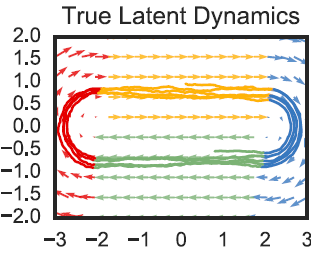
\includegraphics[width=0.35\textwidth]{paper_fig1.png}
	\caption{True dynamics of synthetic NASCAR}
	\label{trueNascar}
\end{figure}

Figure \ref{Nascargen} shows the states generated by both the SLDS and rSLDS fitting of the data. We can see that the rSLDS far outperformed the SLDS. This makes sense because the data was actually generated from an rSLDS, which the SLDS model will not be able to capture. Although this is just simulated data, this proof of concept demonstrates that if the data does indeed come from an SLDS or rSLDS, the approach from the paper will generate a reasonable interpretation of that data.

\begin{figure}[h!]
	\centering
	\begin{subfigure}[b]{0.35\textwidth}
		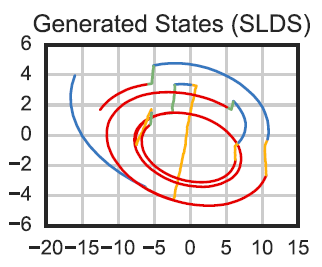
\includegraphics[width=\textwidth]{paper_fig3.png}
		\caption{SLDS}
	\end{subfigure}
	\begin{subfigure}[b]{0.35\textwidth}
		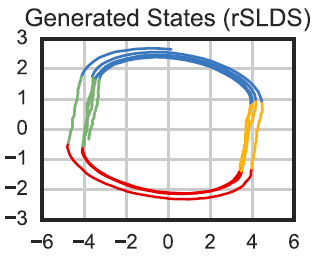
\includegraphics[width=\textwidth]{paper_fig4.png}
		\caption{rSLDS}
	\end{subfigure}
	\caption{Generated states of fit data for synthetic NASCAR}
	\label{Nascargen}
\end{figure}

The next example the authors considered was a system generated by the Lorenz system, a classical nonlinear dynamical system that exhibits chaotic dynamics, switching between two distinct states. However, rather than using Gaussian observations as in a traditional rSLDS, the authors of the paper apply a generalized linear model to the simulated time series data generated by the differential equations and then apply the logistic function. Finally, they collect 100 Bernoulli observations to use as the data to fit the model on.

\begin{figure}[h!]
	\centering
	\begin{subfigure}[b]{0.35\textwidth}
		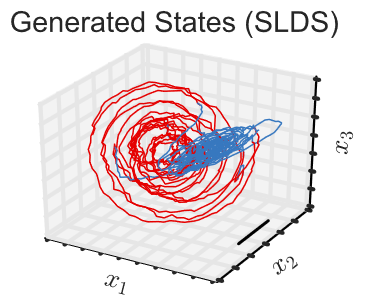
\includegraphics[width=\textwidth]{paper_fig5.png}
		\caption{SLDS}
	\end{subfigure}
	\begin{subfigure}[b]{0.35\textwidth}
		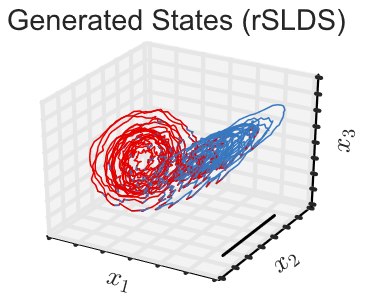
\includegraphics[width=\textwidth]{paper_fig6.png}
		\caption{rSLDS}
	\end{subfigure}
	\caption{Generated states of fit data for the Lorenz data}
	\label{Lorenzgen}
\end{figure}

We can see in Figure \ref{Lorenzgen} that both the SLDS model and the rSLDS model perform reasonably well. The authors found that the rSLDS did perform slightly better than the standard SLDS.

Finally, the authors analyzed data from real basketball players. The data used to fit the model were trajectories from five players in an NBA game between the Miami Heat and the Brooklyn Nets. Rather than an rSLDS, the authors fit the data to a recurrent autoregressive HMM (rAR-HMM), another generalization of the SLDS, where instead of passing through observations of the underlying continuous states, the continuous states are observed directly. These states are assumed to be generated by $K$ latent discrete states. The authors present a subset of these states, and labels them with names of basketball plays that they appear to represent. When comparing these states against those created by a random walk, the predicted states from the recurrent model perform far better; however, there is not evidence that the predicted states capture meaningful patterns in the movements of the players better than the random walk.

\subsection{New Methods}

To reproduce the results of the paper and to apply the models to more systems, we used a more up-to-date approach, as presented in \cite{blei_variational_2017} and \cite{zoltowski_unifying_2020}. These approaches are Black Box Variational Inference (BBVI) and Laplace Variational EM. These models are called state space models (SSMs).

The first approach is based on variational inference, a method from machine learning that approximates probability densities through optimization. The general idea of this approach is to first propose a family of densities that the target data may arise from and find one that generates data close to the target. The ``black box" component of this approach is in reference to a class of these models that avoids any model-specific derivations, so that they can be used for a wide variety of problems. The latter approach combines variational and Laplace approximations over the underlying discrete and continuous variables. The methods for fitting an rSLDS in \cite{linderman_bayesian_2017} using Polya-gamma augmentation are no longer the most up to date. The approaches presented above are more effective at fitting data to an rSLDS.



%%%%%%%%%%%%%%%%%%%%%%%%%%%%%%%%%%%%%%%%%%%%%%%%%%%%%%%
% Make sure to add any new macros to the final report 
% to ensure that they do not conflict with existsing
% ones.
%%%%%%%%%%%%%%%%%%%%%%%%%%%%%%%%%%%%%%%%%%%%%%%%%%%%%%%

\section{Reproduction of Results in the Paper}

Prior to applying the recent methods to new systems, we first explore their potential as inference algorithm for the rSLDS by reproducing the results of \cite{linderman_bayesian_2017}. We compare the Polyagamma approach to the variational inference algorithms by using data from an rSLDS that models the Synthetic NASCAR and solutions simulated from the chaotic Lorenz system.

\subsection{Synthetic NASCAR}

We generate a simulated dataset to represent a non-linear system that aims to imitate cars moving around a track. It consists of four states in total: two for driving along each straight section and two for navigating the semicircular turns at each end of the track. When constructing the rSLDS that models this dataset, we establish transition probabilities based solely on the preceding states. In other words, there is no reliance on the previous state $z_t$. Instead, each state is influenced by a constant bias $r_i$, which steers the transitions toward state $i$. This model is inherently less adaptable compared to the complete rSLDS formulation. Once we have created the rSLDS and generated a trajectory by sampling, we visualize the actual trajectory on a plot.
\begin{figure}[h!]
	\centering
	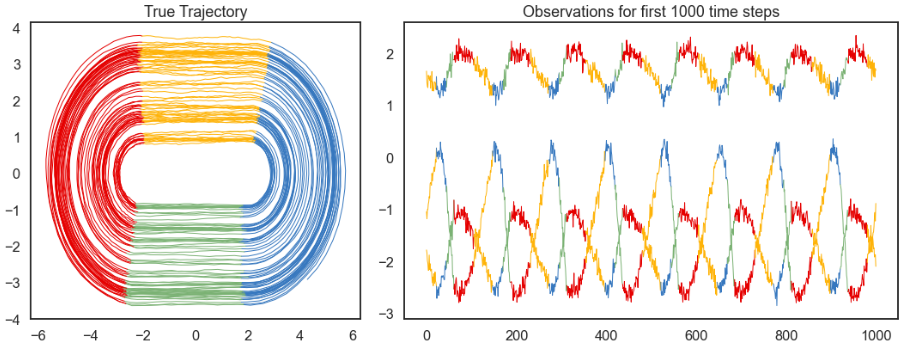
\includegraphics[width=0.75\textwidth]{paper_fig7.png}
	\caption{Exact trajectories of the Nascar model and the evolution of observations during the first 1000 time steps. The true dynamics switch between four states which are indicated by different colors.}
	\label{trueNascar}
\end{figure}

The left panel displays the continuous state trajectories, while the right one presents three observation traces from the first 1000 time steps. Although our observations have ten dimensions, we have plotted only three traces to maintain clarity and reduce visual clutter. Afterward, we proceed to create a new rSLDS object and train it using the data generated previously. It is important to note that this new rSLDS model will only have access to the observations, and it will not be aware of the true states or any other underlying information. By fitting and training the new model, we can recover the behavior of the system up to an affine transformation. The nonlinear behavior is learned by the model however one might still need to apply a rotation to recover the original vector field. This clarifies why the colors of the distinct states may not consistently correspond to the original ones. The behavior of NASCAR was simulated using both BBVI and Laplace EM methods, and the outcomes are presented in Figure \ref{generatedNascar}. It is evident that the estimated latent trajectories obtained through the Laplace EM method exhibit a closer match to the ground truth. Furthermore, the inferred trajectories by either of the variational algorithms demonstrate a closer alignment with the solution when compared to the Polyagamma approach.
\begin{figure}[h!]
	\centering
	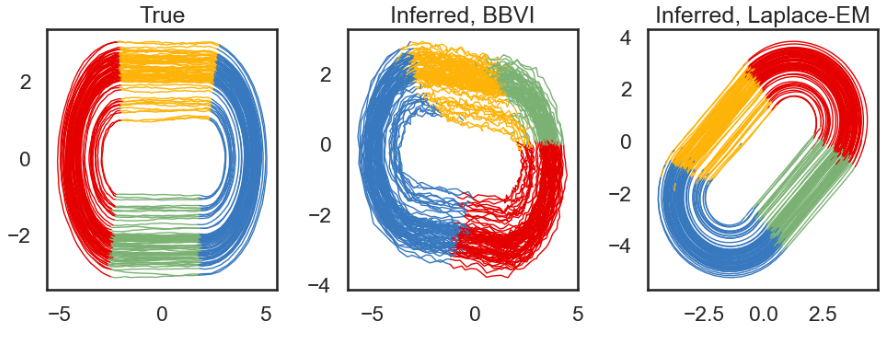
\includegraphics[width=0.75\textwidth]{paper_fig8.png}
	\caption{Generated trajectories of the Nascar model using rSLDS with both BBVI and Laplace EM.}
	\label{generatedNascar}
\end{figure}

\subsection{Lorenz system}
Rather than acquiring data from a linear model with Bernoulli observations, as stated in \cite{linderman_bayesian_2017}, we employ an ODE solver to generate data from a Lorenz system with various initial conditions. To enhance the realism of our data, we introduce perturbations by adding Gaussian noise with a mean of 0 and a variance of 1. We consider the resulting data as observations that would be utilized as input for our rSLDS model. Given the presence of two prominent states within the system, we construct our rSLDS model using 2 discrete states and a continuous latent variable of 3 dimensions. Subsequently, we fit the model to the 4-dimensional observations, and the outcomes for both the BBVI and Laplace EM approaches are condensed in Figure \ref{lorenz}. Regarding this system, both variational algorithms performed exceptionally well in inferring the qualitative behavior, and both yielded more accurate results compared to those discussed in \cite{linderman_bayesian_2017}.
\begin{figure}[h!]
	\centering
	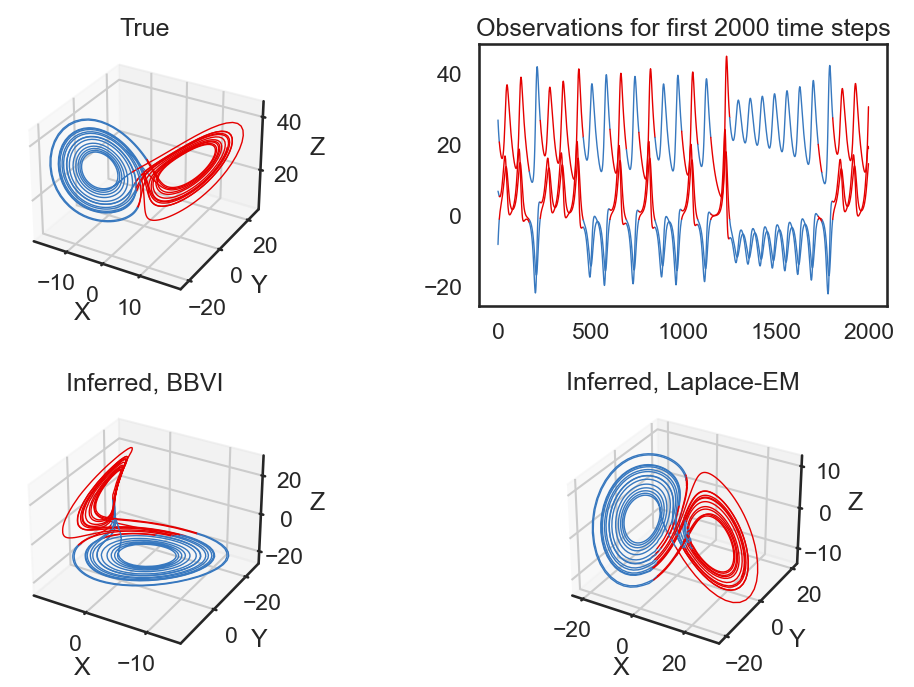
\includegraphics[width=0.75\textwidth]{paper_fig9.png}
	\caption{Qualitative behavior of the Lorenz system and comparison between true and generated states.}
	\label{lorenz}
\end{figure}


\section{Novel Results}
We will continue to extend the rSLDS model using BBVI and Laplace EM inference to dynamical systems exhibiting bifurcations. We wish to see how well the model can recapture the changing dynamics of a fixed point near the bifurcation. First, we will examine the Van der Pol oscillator which has a Hopf bifurcation. Finally, we explored the normal form of the Bautin bifurcation which has a Bautin bifurcation.  
% We continue to look at the R\"ossler attractor which has a period-doubling bifurcation. 

\subsection{Van der Pol Oscillator}
The Van der Pol oscillator is a second-order differential equation of the form
\begin{equation}
    \frac{\ddd^2 x}{\ddd t^2} - \mu(1 - x^2)\frac{\ddd x}{\ddd t} + x = 0,
\end{equation}
where $x$ is the spatial coordinates and $\mu$ is a scalar parameter. The equation can be rewritten into its two-dimensional form using the transformation $y = x_t$ to get
\begin{equation}
    \begin{cases}
        x_t = y,\\
        y_t = \mu(1-x^2)y - x.
    \end{cases}
\end{equation}
Setting $x_t$ and $y_t$ equal to zero, we find that the Van der Pol oscillator has a fixed point at the origin $(x,y) = (0,0)$ which is known to be a Hopf bifurcation. This means that the stability of the fixed point is stable for $\mu < 0$ and there are no limit cycles near the fixed point. When $\mu = 0$, the Van der Pol system becomes linear and the origin is a circular node. Lastly, when $\mu > 0$, the fixed point becomes unstable and a stable limit cycle around the origin appears. We demonstrate the different behaviors in Figure \ref{trueVDP}. On the left $\mu > 0$, the stable limit cycle around the fixed point can be seen. In the middle $\mu =0$, the trajectory forms a circle around the center node. On the right $\mu > 0$, the trajectory spirals into the stable fixed point. 

\begin{figure}
    \centering
    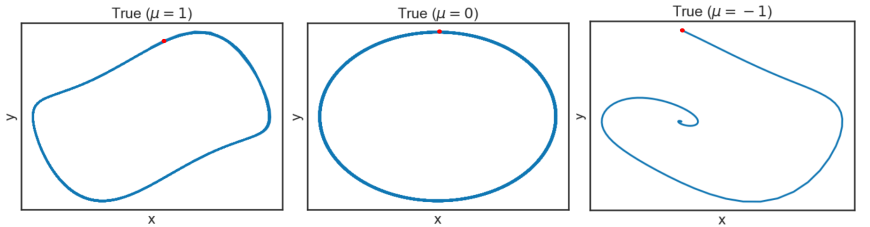
\includegraphics[width=0.90\textwidth,height=\textwidth,keepaspectratio]{./figures/paper_fig10.png}
    \caption{True trajectories used to fit rSLDS model over $T\in[0,1000]$ with $1000$ observations. The initial condition of $(0,2.2)$ can be seen in red. On the left, $\mu =1$ and the stable limit cycle can be seen. In the middle, $\mu = 0$ and the fixed point is a center. On the right, $\mu = -1$ and the fixed point is stable.}
    \label{trueVDP}
\end{figure}

To fit the Van der Pol oscillator to the rSLDS model, we use an ODE solver to generate data from the Lorenz system at a fixed initial condition $(x,y) = (0,2)$ and $t \in [0,1000]$ using $10000$ observations. To study how the model handles bifurcations, we sample the trajectory when $\mu = -1,0,1$ which are around and on the bifurcation. The true trajectories that are used to train the model can be seen in Figure \ref{trueVDP}. Once again, we enhance the realism of our data by adding Gaussian noise. In the $\mu = 1$ case, we expect a stable limit cycle that has two prominent states and thus we construct the model using two discrete states. For the sake of consistency, we set the model to have two discrete states for each $\mu$ value. 

\begin{figure}
    \begin{subfigure}[b]{0.33\linewidth}
        \centering
        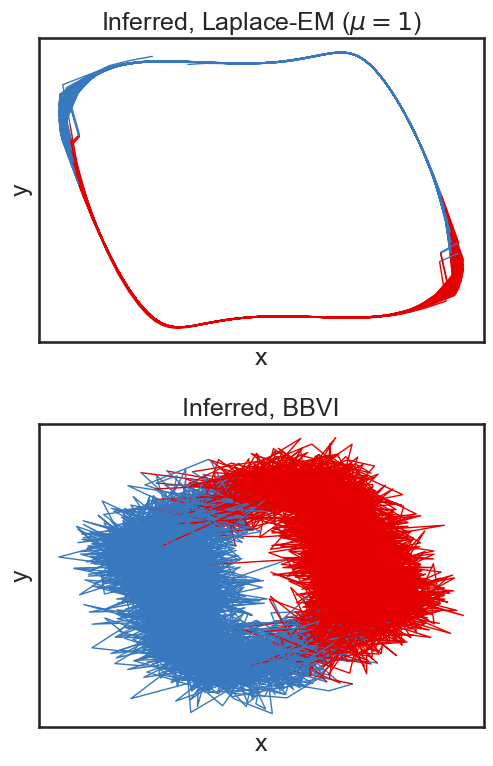
\includegraphics[width=\linewidth]{./Figures/vdp-bad-mu1.png}
        \caption{}
        \label{badvdp:a}
        \vspace{4ex}
    \end{subfigure}%%
    \begin{subfigure}[b]{0.33\linewidth}
        \centering
        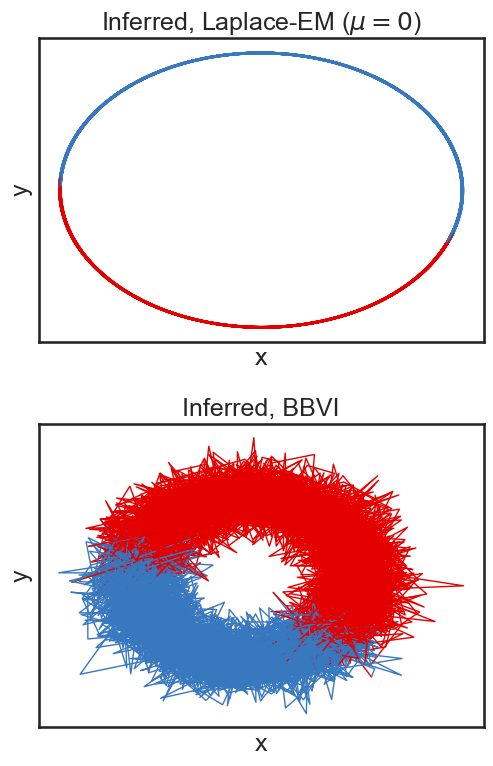
\includegraphics[width=\linewidth]{./Figures/vdp-bad-mu0.png}
        \caption{}
        \label{badvdp:b}
        \vspace{4ex}
    \end{subfigure}%%
    \begin{subfigure}[b]{0.33\linewidth}
        \centering
        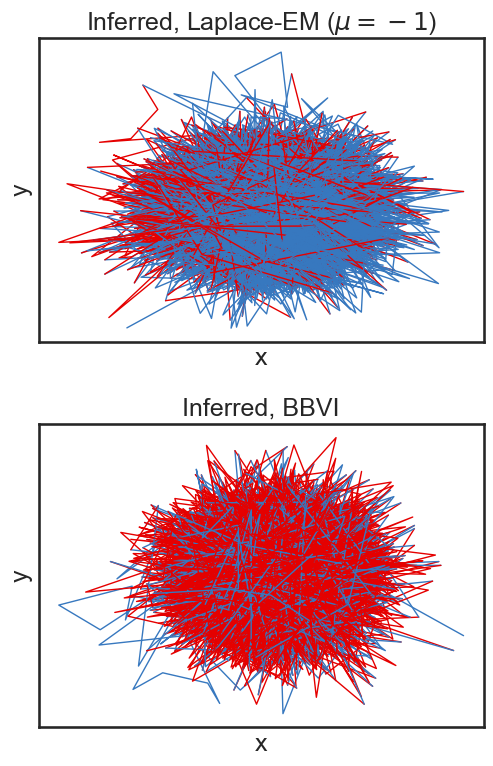
\includegraphics[width=\linewidth]{./Figures/vdp-bad-mu-1.png}
        \caption{}
        \label{badvdp:c}
        \vspace{4ex}
    \end{subfigure}
    \caption{Recovered trajectories from rSLDS model using the Laplace-EM and BBVI methods with Gaussian noise present. In (A), $\mu = 1$ and the Laplace-EM recovers the system with two latent states, seen in blue and red, but BBVI has a high amount of noise. In (B), $\mu = 0$ and the same results occur as in (A). In (C), $\mu = -1$ and both methods fail to recover the true behavior.}
    \label{badvdp}
\end{figure}

By fitting and training an rSLDS model for each $\mu$ value using the BBVI and Laplace EM methods, we recover the trajectories of the original system which are presented in Figure \ref{badvdp}. While the rSLDS model was able to recover the trajectories for the $\mu=0,1$ case, the model failed to rediscover the behavior at $\mu = -1$. To handle this, we turn down the amount of Gaussian noise being added to the observations. Retraining the model we recover the dynamics of the $\mu = -1$ as seen in Figure \ref{goodvdp}. When comparing the results to the true trajectories, we see that for each $\mu$ value, the rSLDS models using Laplace EM and BBVI are both able to accurately recover the behavior of the Van der Pol system near the bifurcation. When $\mu = 1$, both models identify two latent states exceptionally well. In the $\mu = 0$ case, although the BBVI method struggles to identify the latent states by overlapping the latent states, the Laplace EM model identifies one latent state for the entire trajectory. On the other hand, when $\mu = -1$ both methods struggle to identify the latent states.

\begin{figure}
    \begin{subfigure}[b]{0.33\linewidth}
        \centering
        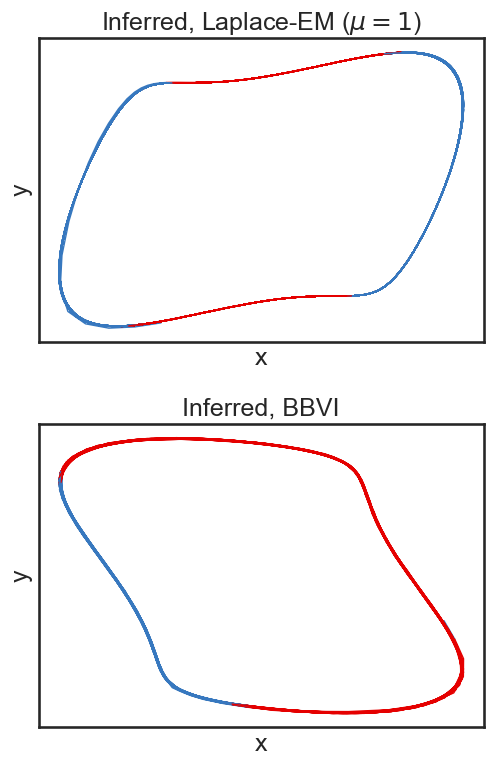
\includegraphics[width=\linewidth]{./Figures/vdp-good-mu1.png}
        \caption{}
        \label{goodvdp:a}
        \vspace{4ex}
    \end{subfigure}%%
    \begin{subfigure}[b]{0.33\linewidth}
        \centering
        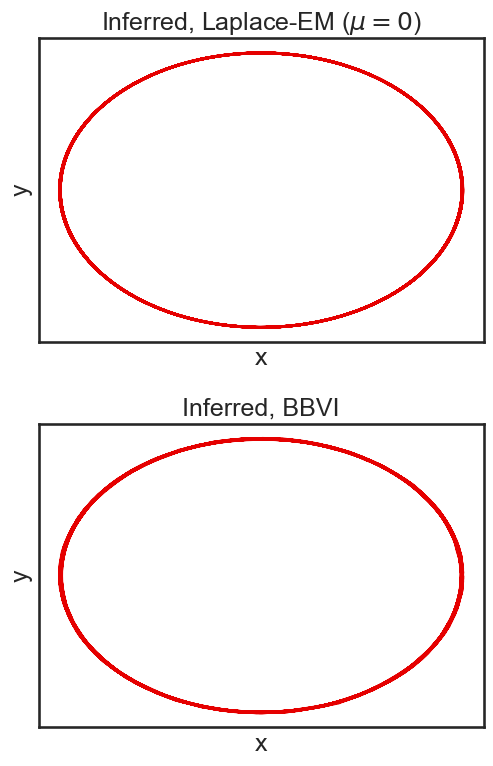
\includegraphics[width=\linewidth]{./Figures/vdp-good-mu0.png}
        \caption{}
        \label{goodvdp:b}
        \vspace{4ex}
    \end{subfigure}%%
    \begin{subfigure}[b]{0.33\linewidth}
        \centering
        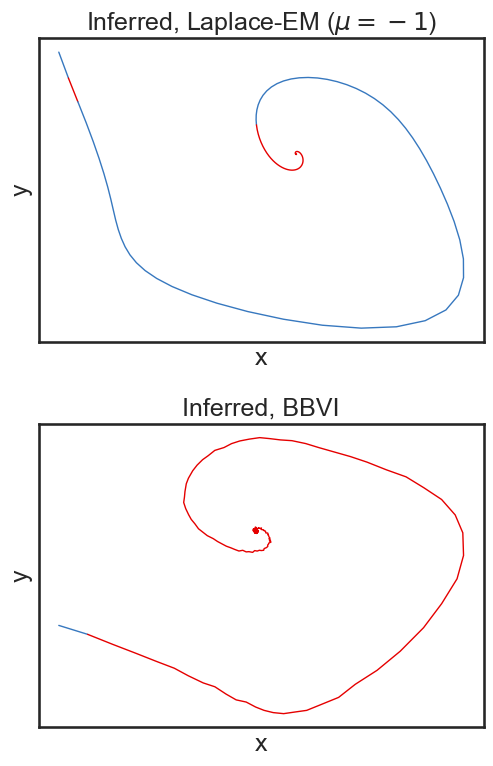
\includegraphics[width=\linewidth]{./Figures/vdp-good-mu-1.png}
        \caption{}
        \label{goodvdp:c}
        \vspace{4ex}
    \end{subfigure}
    \caption{Recovered trajectories from rSLDS model using the Laplace-EM and BBVI methods with a low amount of Gaussian noise present. In (A), $\mu = 1$ and while both methods accurately recover the true trajectories, Laplace-EM places the latent states with higher accuracy. In (B), $\mu = 0$ and the same results occur as in (A). While from the graph it is not evident, BBVI fails to place the latent states accurately and rather overlaps them. In (C), $\mu = -1$ and both methods fail to recover the latent states that are insightful.}
    \label{goodvdp}
\end{figure}

\subsection{Bautin Bifurcation}
We extend our examination of bifurcations to see how the models handle a generalized Hopf bifurcation. Consider the autonomous system of ordinary differential equations
\begin{equation}
    \dot{y} = f\paren{y, \beta},
\end{equation}
where $y = (y_1,y_2)^T \in \R^2$ are the spatial coordinates and the system depends upon $\beta = (\beta_1,\beta_2) \in \R^2$. Supposing the system has a fixed point on the origin, the fixed point is said to experience a generalized Hopf bifurcation known as a Bautin bifurcation if specific conditions upon the first and second Lypanonuv coefficients, the details are omitted as they are not deemed insightful to the paper. When these conditions are met, $\dot{y}$ is locally equivalent near the origin to 
\begin{equation}
    \begin{cases}
        \dot{y_1} = \beta_1 y_1 - y + \beta_2 y_1 \paren{y_1^2 + y^2} + \sigma y_1 \paren{y_1^2 + y^2}^2,\\
        \dot{y_2} = y_1 + \beta_1 y + \beta_2 y \paren{y_1^2 + y^2} + \sigma y \paren{y_1^2 + y^2}^2,
    \end{cases}
\end{equation}
which is the normal form of the Bautin bifurcation. Here $\sigma = \pm 1$ is related to the sign of the first Lypanonuv coefficient. 


\begin{figure}
    \centering
    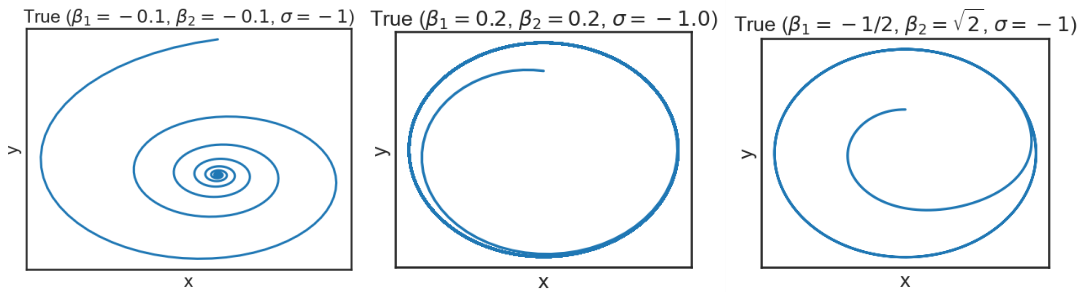
\includegraphics[width=0.9\textwidth,height=\textwidth,keepaspectratio]{./Figures/bautin-true.png}
    \caption{True trajectories used to fit rSLDS model over $T\in[0,1000]$ with $1000$ observations. The initial condition of $(0,0.55)$ and $\sigma = -1$ is used for each trajectory. On the left, $\beta_1 = \beta_2 = -0.1$ and the trajectory spirals into the stable fixed point away from the unstable limit cycle. In the middle, $\beta_1 = \beta_2 = 0.2$ and the trajectory moves away from the unstable fixed point and into the stable limit cycle. On the right $\beta_1 = -1/2$ and $\beta_2 = \sqrt{2}$ and the trajectory spirals away from the unstable limit cycle on the inside and towards the stable limit cycle on the outside. }
    \label{bautin-true}
\end{figure}


For the work of the paper, we will consider $\dot{y}$ to be the normal form of the Bautin bifurcation and observe how the system handles the three following behaviors around the bifurcation point. When $\beta_1,\beta_2 < 0$, the origin is stable with an unstable limit cycle around it. When $\beta_1,\beta_2 > 0$, the fixed point becomes stable and the limit cycle around unstable. In the specific subregion of $-1/4 \beta_2^2 < \beta_1 < 0$ and $\beta_2>0$, a second limit cycle emerges around the stable fixed point. The outer limit cycle is stable while the inner limit cycle is unstable. We demonstrate this behavior in Figure \ref{bautin-true}. On the left, $\beta_1 = \beta_2 < 0$ and the trajectory spirals into the stable fixed point and away from the unstable limit cycle. In the middle $\beta_1 = \beta_2 > 0$ and the trajectory travels to the stable limit cycle away from the unstable fixed point. On the right, $\beta_1 = -1/4 \beta_2^2$ and $\beta_2 > 0$ and we see the trajectory spiraling away from the unstable limit cycle into the stable limit cycle. 

To fit the Bautin system to the rSLDS model, we follow the same procedure as outlined for the Van der Pol. We will once again use an ODE solver on $\dot{y}$ for a fixed initial condition $(y_1,y_2) = (0,0.55)$ and $t\in[0,1000]$ using 10000 observations to create the sample data for the model. We used parameter values $(\beta_1,\beta_2) \in \left\{(-0.1,-0.1),(0.2,0.2),\left(-1/2,\sqrt{2}\right)\right\}$ which are near the Bautin bifurcation to get the true trajectories seen in Figure \ref{bautin-true}. Note that once again, the amount of noise added to the system is reduced to help the rSLDS model rediscover the dynamics. Fitting the rSLDS model using BBVI and Laplace EM, both methods recover the dynamics near the bifurcation point up to an affine transformation as seen in Figure \ref{bautinresults}. When $(\beta_1,\beta_2) = (-0.1,-0.1)$, both methods capture the dynamics of the stable fixed point although the BBVI results are less smooth. When $(\beta_1,\beta_2) = (0.2,0.2)$, both methods recover the stable limit cycle. Finally, when $(\beta_1,\beta_2) = (-1/2,\sqrt{2})$, both methods show the presence of an unstable limit cycle within a stable limit cycle. In each of the cases, both the Laplace EM and BBVI methods struggled to place two latent spaces and so we omitted the colors of the different states from the figure.  

\subsection{Remarks}
For both the methods, Laplace EM and BBVI, of the rSLDS model, the model accurately rediscovers the local dynamics near and on the bifurcation point but struggles to place two latent states in meaningful positions. More specially, fitting the model to the Van der Pol oscillator near the Hopf bifurcation highlights how the Laplace EM method outperforms the BBVI method at smoothly recreating the dynamics of the trajectory. Here the Laplace EM method is also able to place meaningful latent states for two of the cases near the bifurcation. Fitting the model to the Bautin system once again shows that the Laplace method outperforms the BBVI. Nevertheless, in both situations, the rSLDS model is only able to fit the dynamics of the model accurately when there is a low amount of noise present in the observation data.

\begin{figure}
    \begin{subfigure}[b]{0.33\linewidth}
        \centering
        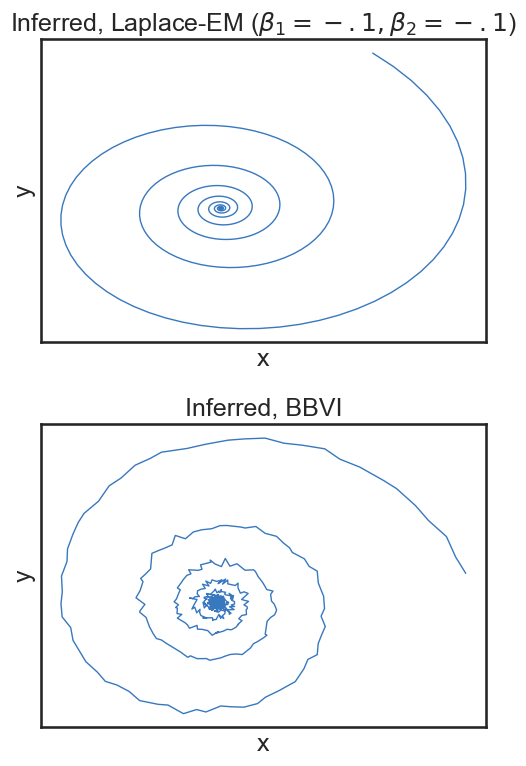
\includegraphics[width=\linewidth]{./Figures/bautin-stable.png}
        \caption{}
        \label{bautinresults:a}
        \vspace{4ex}
    \end{subfigure}%%
    \begin{subfigure}[b]{0.33\linewidth}
        \centering
        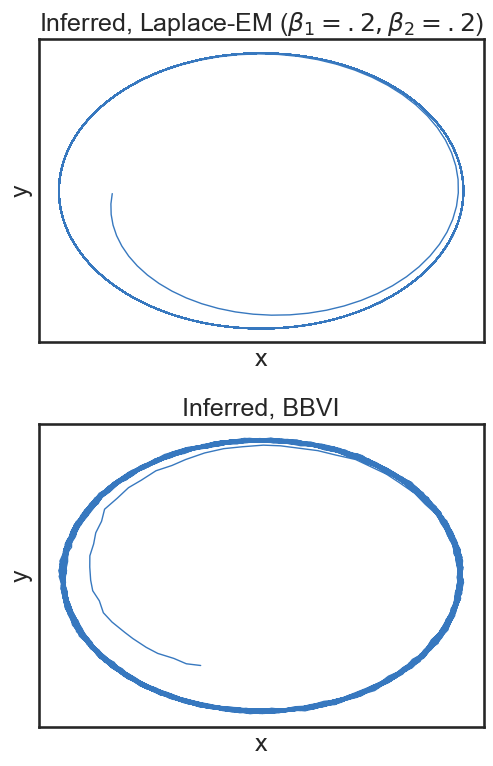
\includegraphics[width=\linewidth]{./Figures/bautin-unstab.png}
        \caption{}
        \label{bautinresults:b}
        \vspace{4ex}
    \end{subfigure}%%
    \begin{subfigure}[b]{0.33\linewidth}
        \centering
        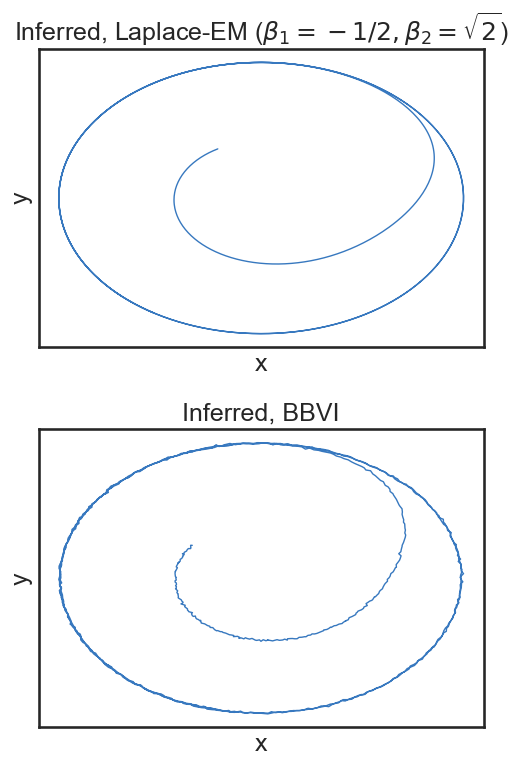
\includegraphics[width=\linewidth]{./Figures/bautin-lpc.png}
        \caption{}
        \label{bautinresults:c}
        \vspace{4ex}
    \end{subfigure}
    \caption{Recovered trajectories from the rSLDS model using the Laplace-EM and BBVI methods with a low amount of Gaussian noise present. In (A), $\beta_1 = \beta_2 = -0.1$ and the Laplace-EM method smoothly recovers the true trajectory while the BBVI recovers a trajectory with noise. In (B), $\beta_1 = \beta_2 = 0.2$ and both methods perform similarly to (A). Note that once again it can be seen that the BBVI has more noise due to the variance (thickness of the line) of the limit cycle. In (C) $\beta_1 = -1/2$ and $\beta_2 = \sqrt{2}$ and the same results from (A) and (B) occur.}
    \label{bautinresults}
\end{figure}

\section{Conclusions}

The rSLDS model, in all the cases that we examined, was able to capture the dynamics of complex canonical dynamical systems, at least under certain conditions. When the dynamics of the underlying system feature a stable fixed point or an unstable orbit, the model is only able to reproduce the dynamics if the noise on the observations is sufficiently small. However, if the system exhibits a stable orbit or limit cycle, the rSLDS model is particularly effective at reproducing the dynamics of the underlying system.

Another potential downside of this model is that it is only able to reproduce the dynamics associated with a single trajectory, at least with the current fitting methods. Since the model depends on time series data, we cannot append multiple trajectories in the same system to fit the model for broader initial conditions. This makes the method limited in learning the global dynamics and showing where the boundaries of stability are especially the position of unstable fixed points and periodic orbits.

\begin{comment}
The method can be very successfully applied to systems with a periodic orbit or strange attractor and the goal is to find the dynamics of this orbit. We can remark that this method is very limited in its ability to give an estimation on linear estimation the global dynamics. Unlike the SINDY algorithm \cite{} it is currently not possible to learn from data from multiple trajectories. This makes the method limited in learning the global dynamics and showing where the boundaries of stability are especially the position of unstable fixed points and periodic orbits. This makes the method only applicable for initial conditions that lead to periodic or bounded trajectories. The extension of implementing the ability to handle multiple trajectories will enhance the range of problems this method can be applied to.
\end{comment}


\nocite{linderman_bayesian_2017, zoltowski_unifying_2020, chen_estimating_2015, blei_variational_2017, linderman_dependent_2015}
\bibliographystyle{plain}
\bibliography{bibfile}
\section{Appendix}

All the code used to generate the figures in this report can be found here: 

\href{https://github.com/rohingilman/AMATH575-rSLDSs}{https://github.com/rohingilman/AMATH575-rSLDSs}

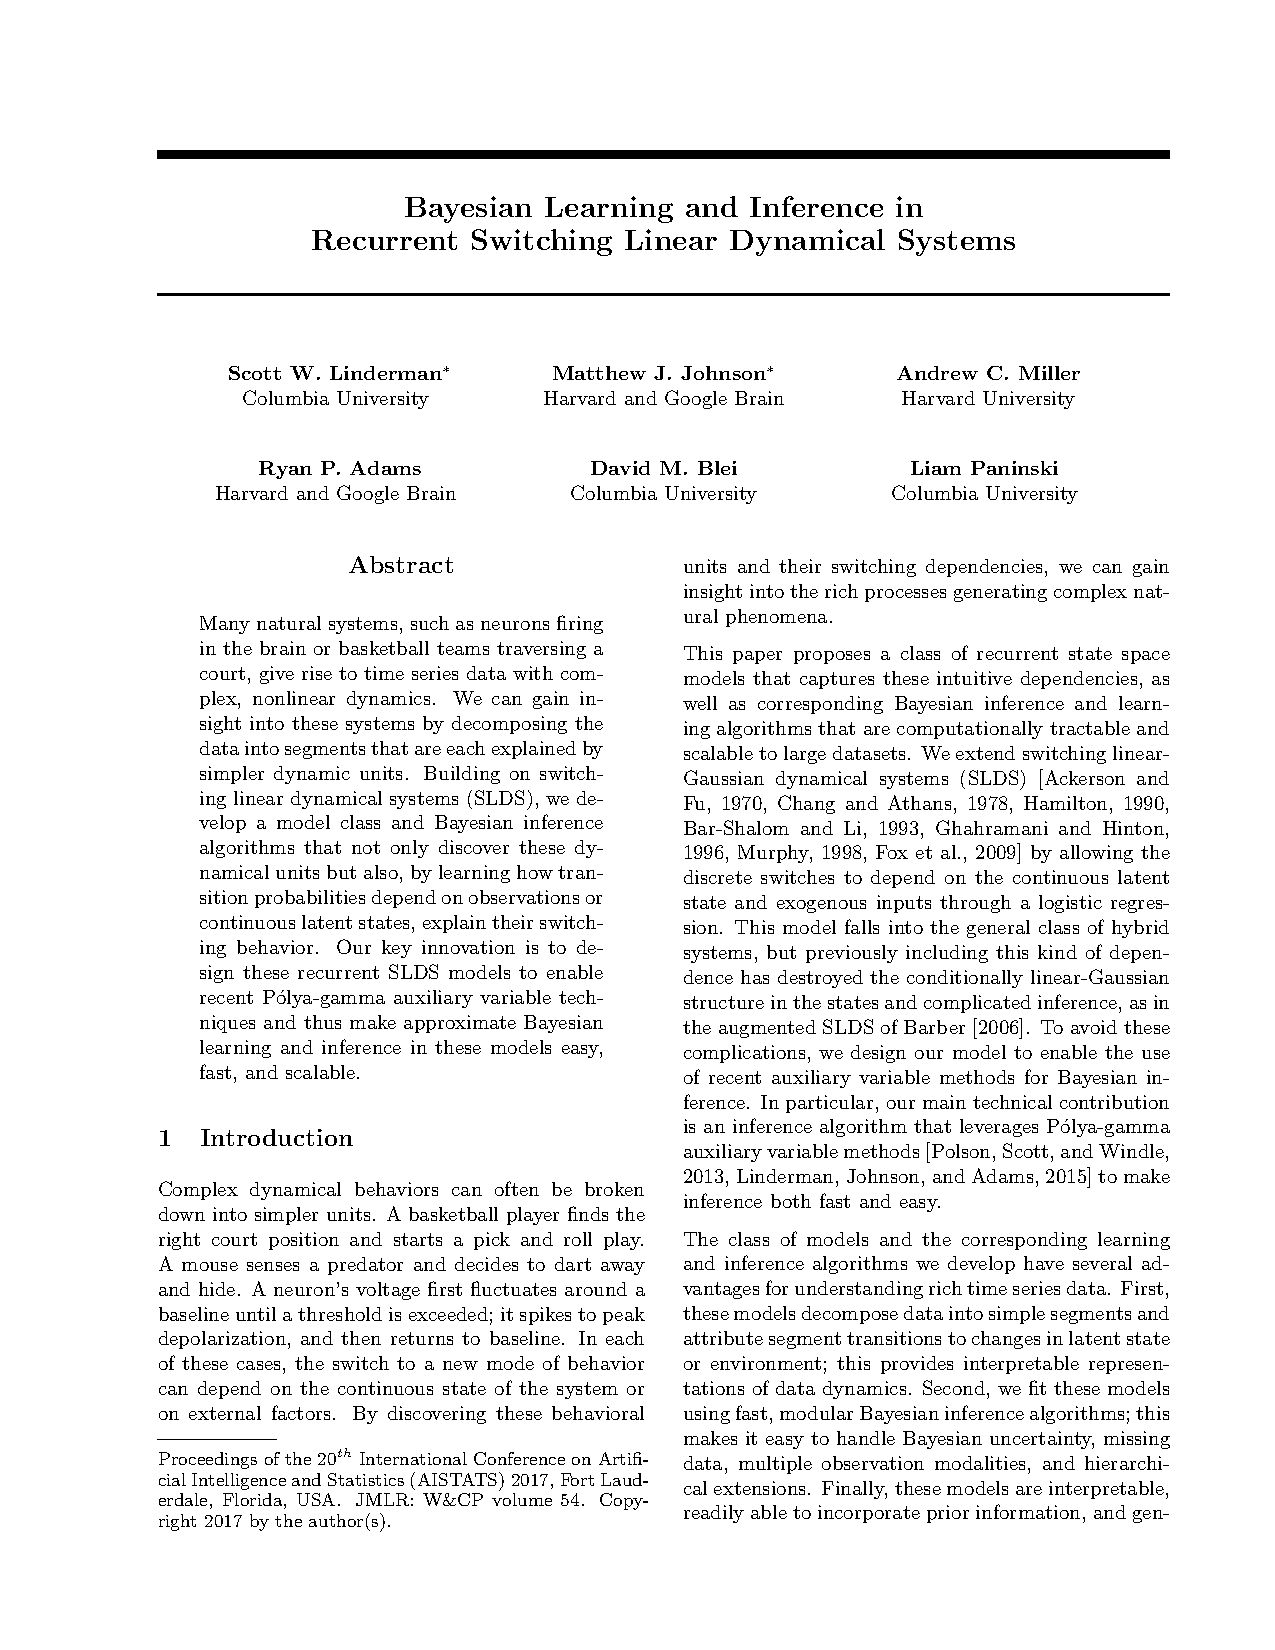
\includepdf[pages=-]{linderman17a.pdf}

\end{document}